\section{Data exploration}

Fluorescent Neuronal Cells images are high-resolution RGB pictures of constant shape (1200 pixels height by 1600 pixels width) collected under fixed experimental conditions.
In terms of features, the data can be explored at two complementary levels. 
In fact, interesting insights can be retrieved by looking at the color and luminance information carried by pixels. Also, conducting analogous analyses on the ground-truth masks reveals

% In terms of data features, the most interesting aspects regard the color and luminance information, the counts distribution and the cells characteristics.
% In terms of data features, the most interesting aspects pertain the color and luminance information, the counts' distribution and characteristics of the cells.
The data can be explored at two complementary levels: pixels features and cells characteristics. 
On the one hand, interesting insights can be retrieved by looking at pixels' color and luminance information. Also, analogous analyses on the ground-truth masks reveal essential information about class-imbalance between signal and background.
On the other hand, examining object properties can highlight potential nuisances and suggest how to evaluate model performances.

\subsection{Graphical features}
% As far as the color, t
The picture appearance is dominated by two prevalent tints due to the intentional selection of a specific wavelength: a darker hue corresponding to areas whose light was filtered out and a yellow tone emitted by the fluorophore
(\cref{fig:dataset:empty,fig:artifacts:clumping}).
As a consequence, the only color channels to be populated are red and green, while blue is typically empty. 
An example of this effect is reported in \cref{fig:dataset:pixel_intensity}, where the average distribution of pixel intensity is illustrated.
\begin{figure}
    \centering
    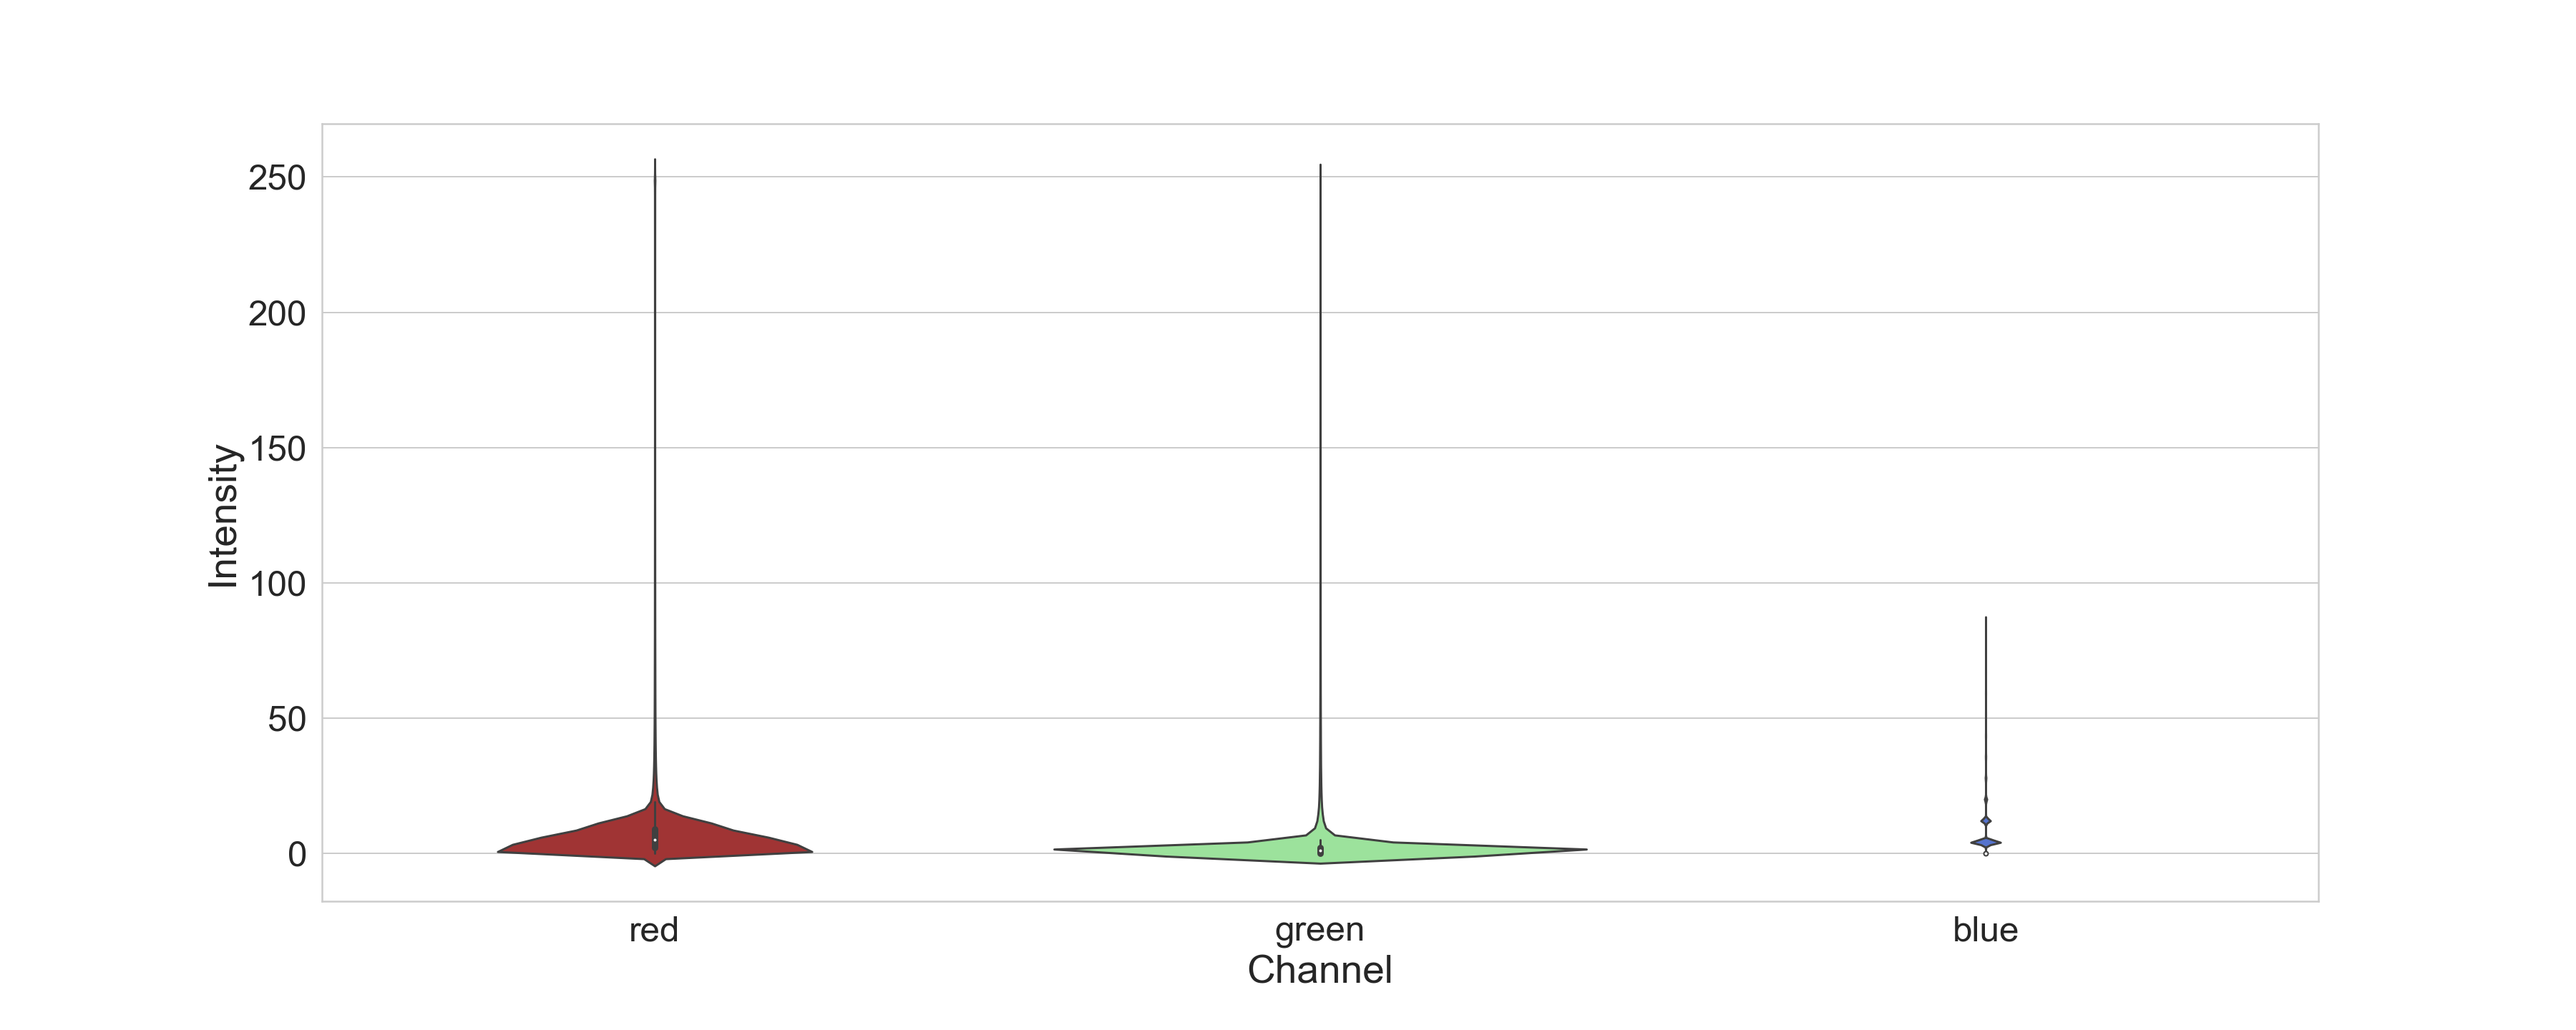
\includegraphics[width=\textwidth]{figures/120_dataset/pixel_intensity_distribution.png}
    \caption{Pixel intensity distribution. Violin plot of the average distribution of pixel intensities across the  RGB channels}
    \label{fig:dataset:pixel_intensity}
\end{figure}
Guided by this observation, one may argue that all this information is superfluous and resorting to a grayscale representation could be better since the images are ultimately shades of yellow.
\Cref{fig:dataset:colorspace} (left) corroborates this intuition, as most pixels lay almost on a straight line in the red-green plane. 
This suggests that the two channels are highly correlated, so a one-dimensional subspace may be enough to represent most of the variability of the data.
In turn, this would bring two advantages: ease the learning process -- as neural networks typically suffer when inputs are correlated %\cite{} 
-- and make it more efficient -- as one considers only one channel instead of three.

However, the use-case at hand has no stringent requirements in terms of computing resources and runtime, so the 3-channels training is still feasible.
More importantly, the information thrown away when converting to grayscale, although tiny, may still be crucial to discriminate background and signal. 
At the same, the RGB colorspace may not be the optimal representation to learn this separation. For instance, \cref{fig:dataset:colorspace} (right) shows the same images according to a different encoding, HSV. 
In this case, the separation between dark and colored tones appears more evident. 
Moreover, most of the pixels are concentrated in low hue values
and their distribution seems more spread across the saturation-value plane. 

All that being considered, this work tried to leverage the insights of both approaches. 
On one side, the RGB colorspace was taken as a starting point to exploit all available information. On the other side, the model first layer was designed to incorporate a colorspace transformation from RGB to a single channel.
% In this way, the intent is to avoid introducing any colorspace-related bias by letting the model learn the most convenient representation and, at the same time, benefit from the computational advantage due to a lower dimensionality.
The intent is to avoid introducing any colorspace-related bias by letting the model learn the most convenient representation without ignoring the fact that a one-dimensional manifold is probably enough to express the variability of the data.
\begin{figure}
    \centering
    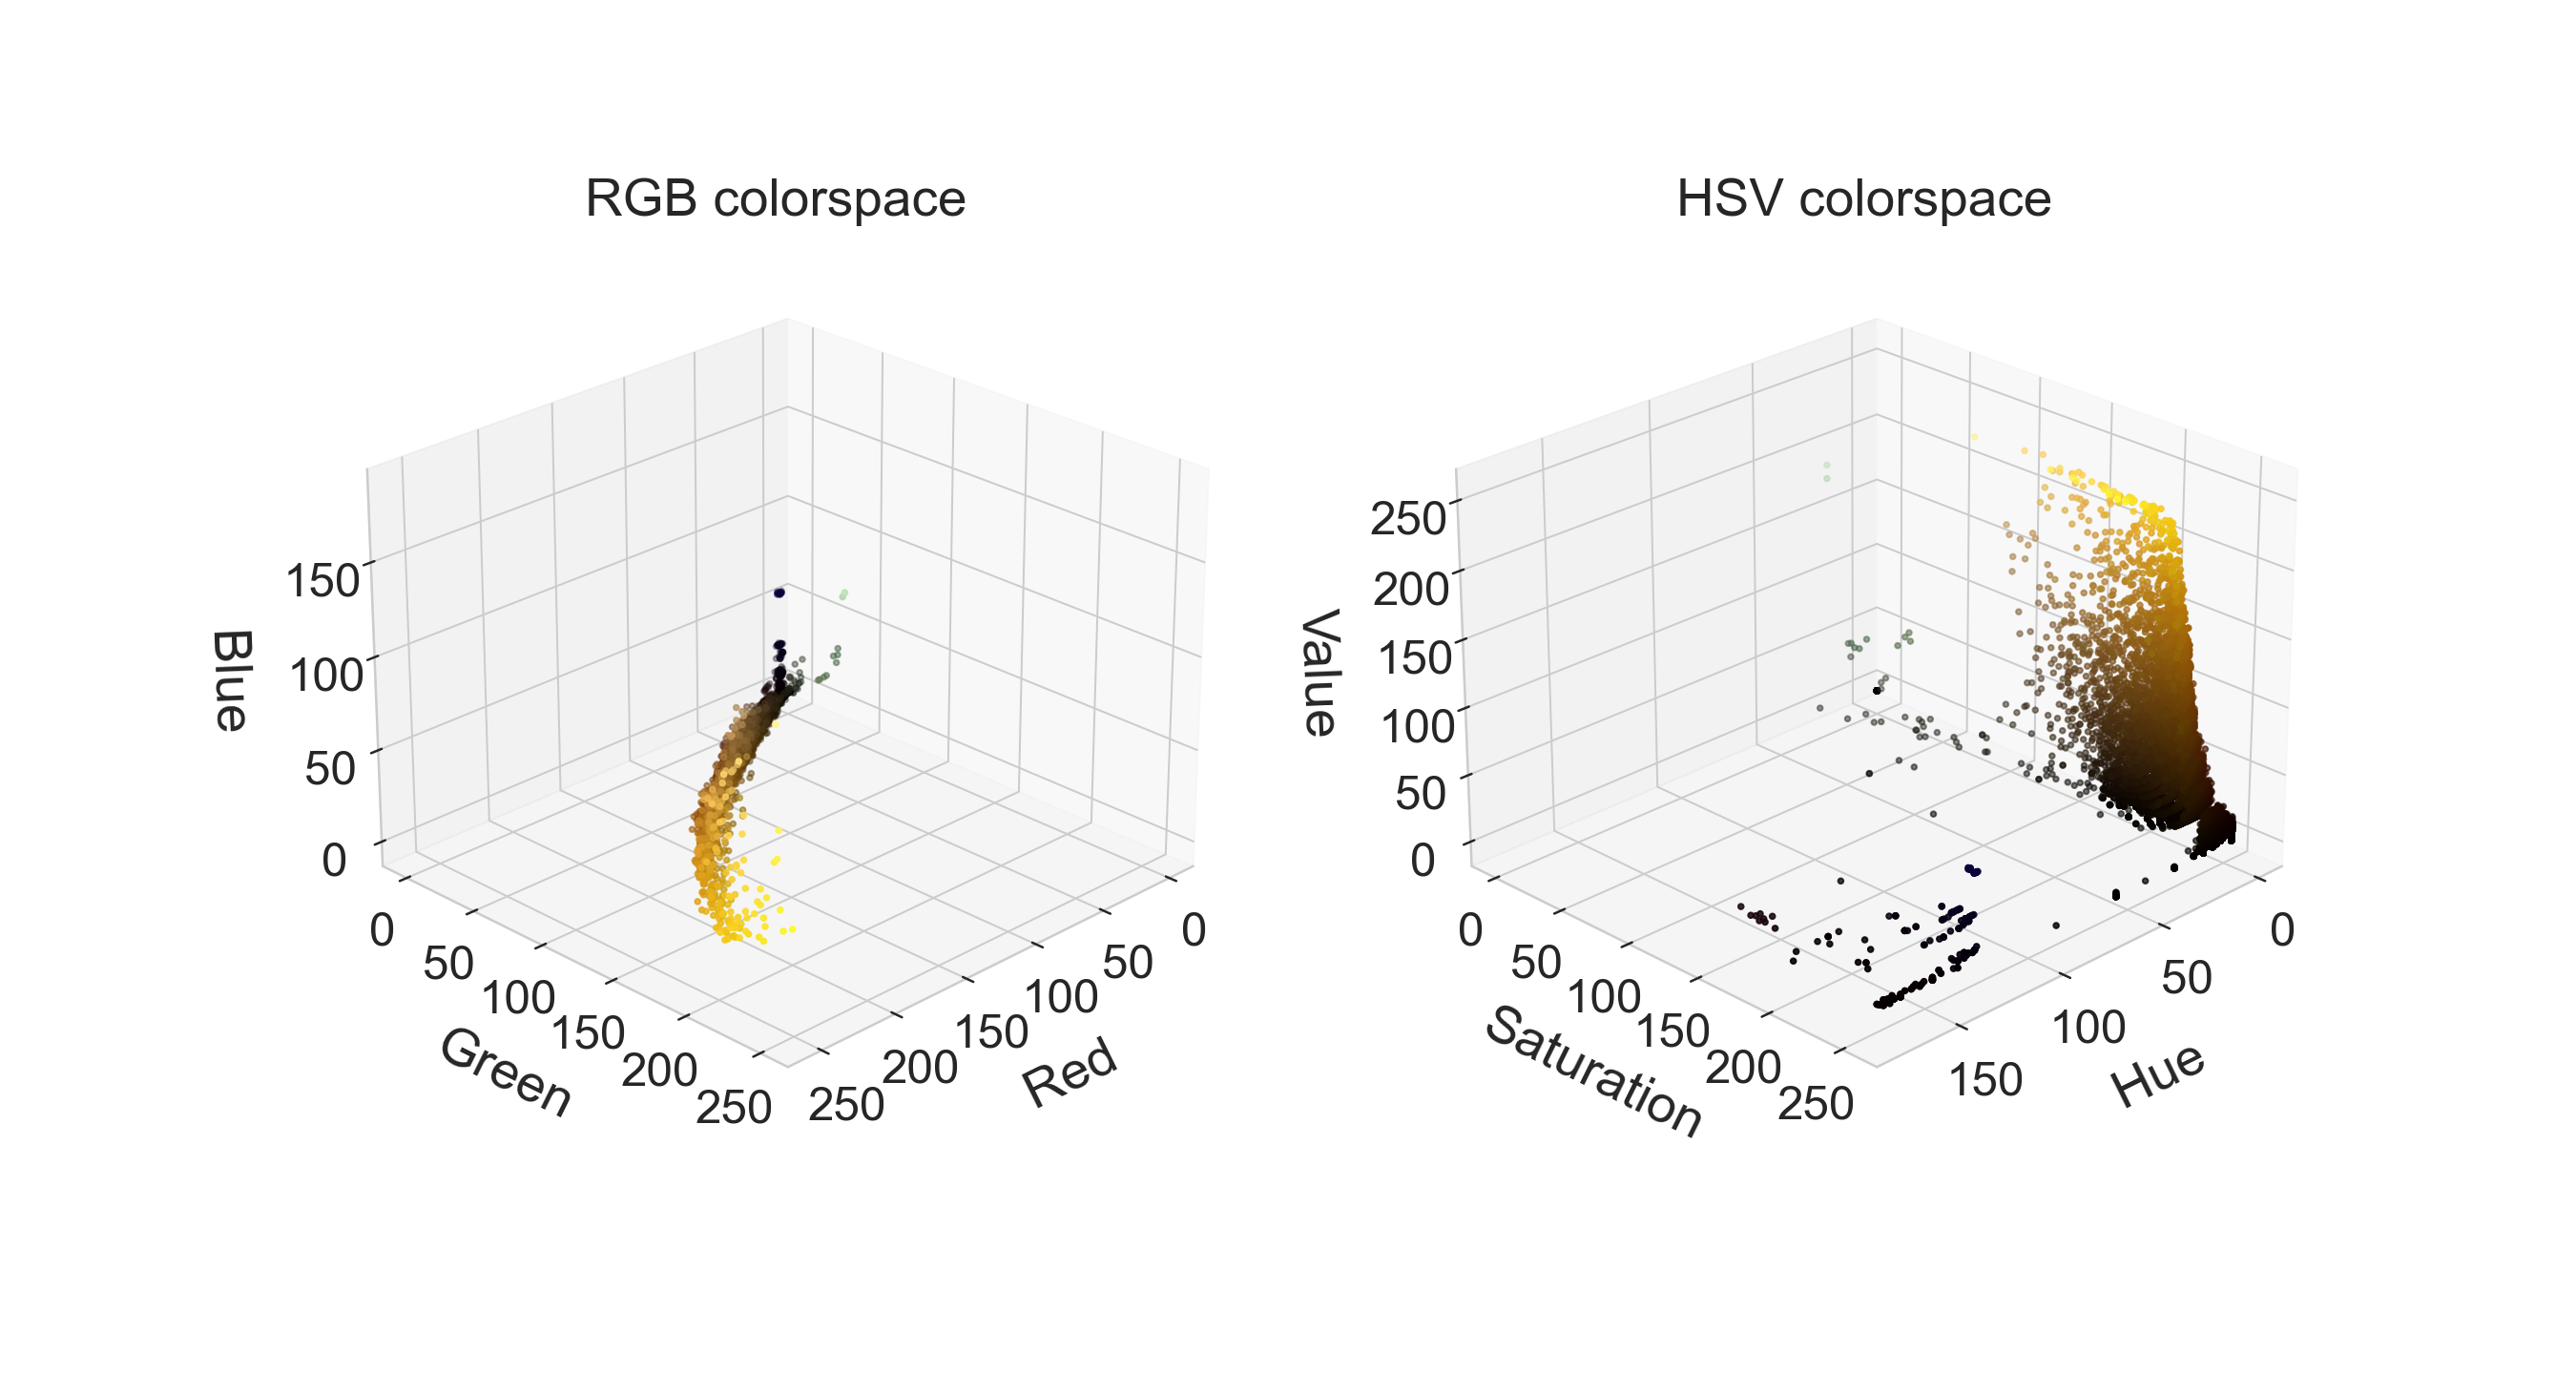
\includegraphics[width=1.1\textwidth]{figures/120_dataset/colorspace_Mar23bS1C2R3_VLPAGl_200x_y.png}
    
    \centering
    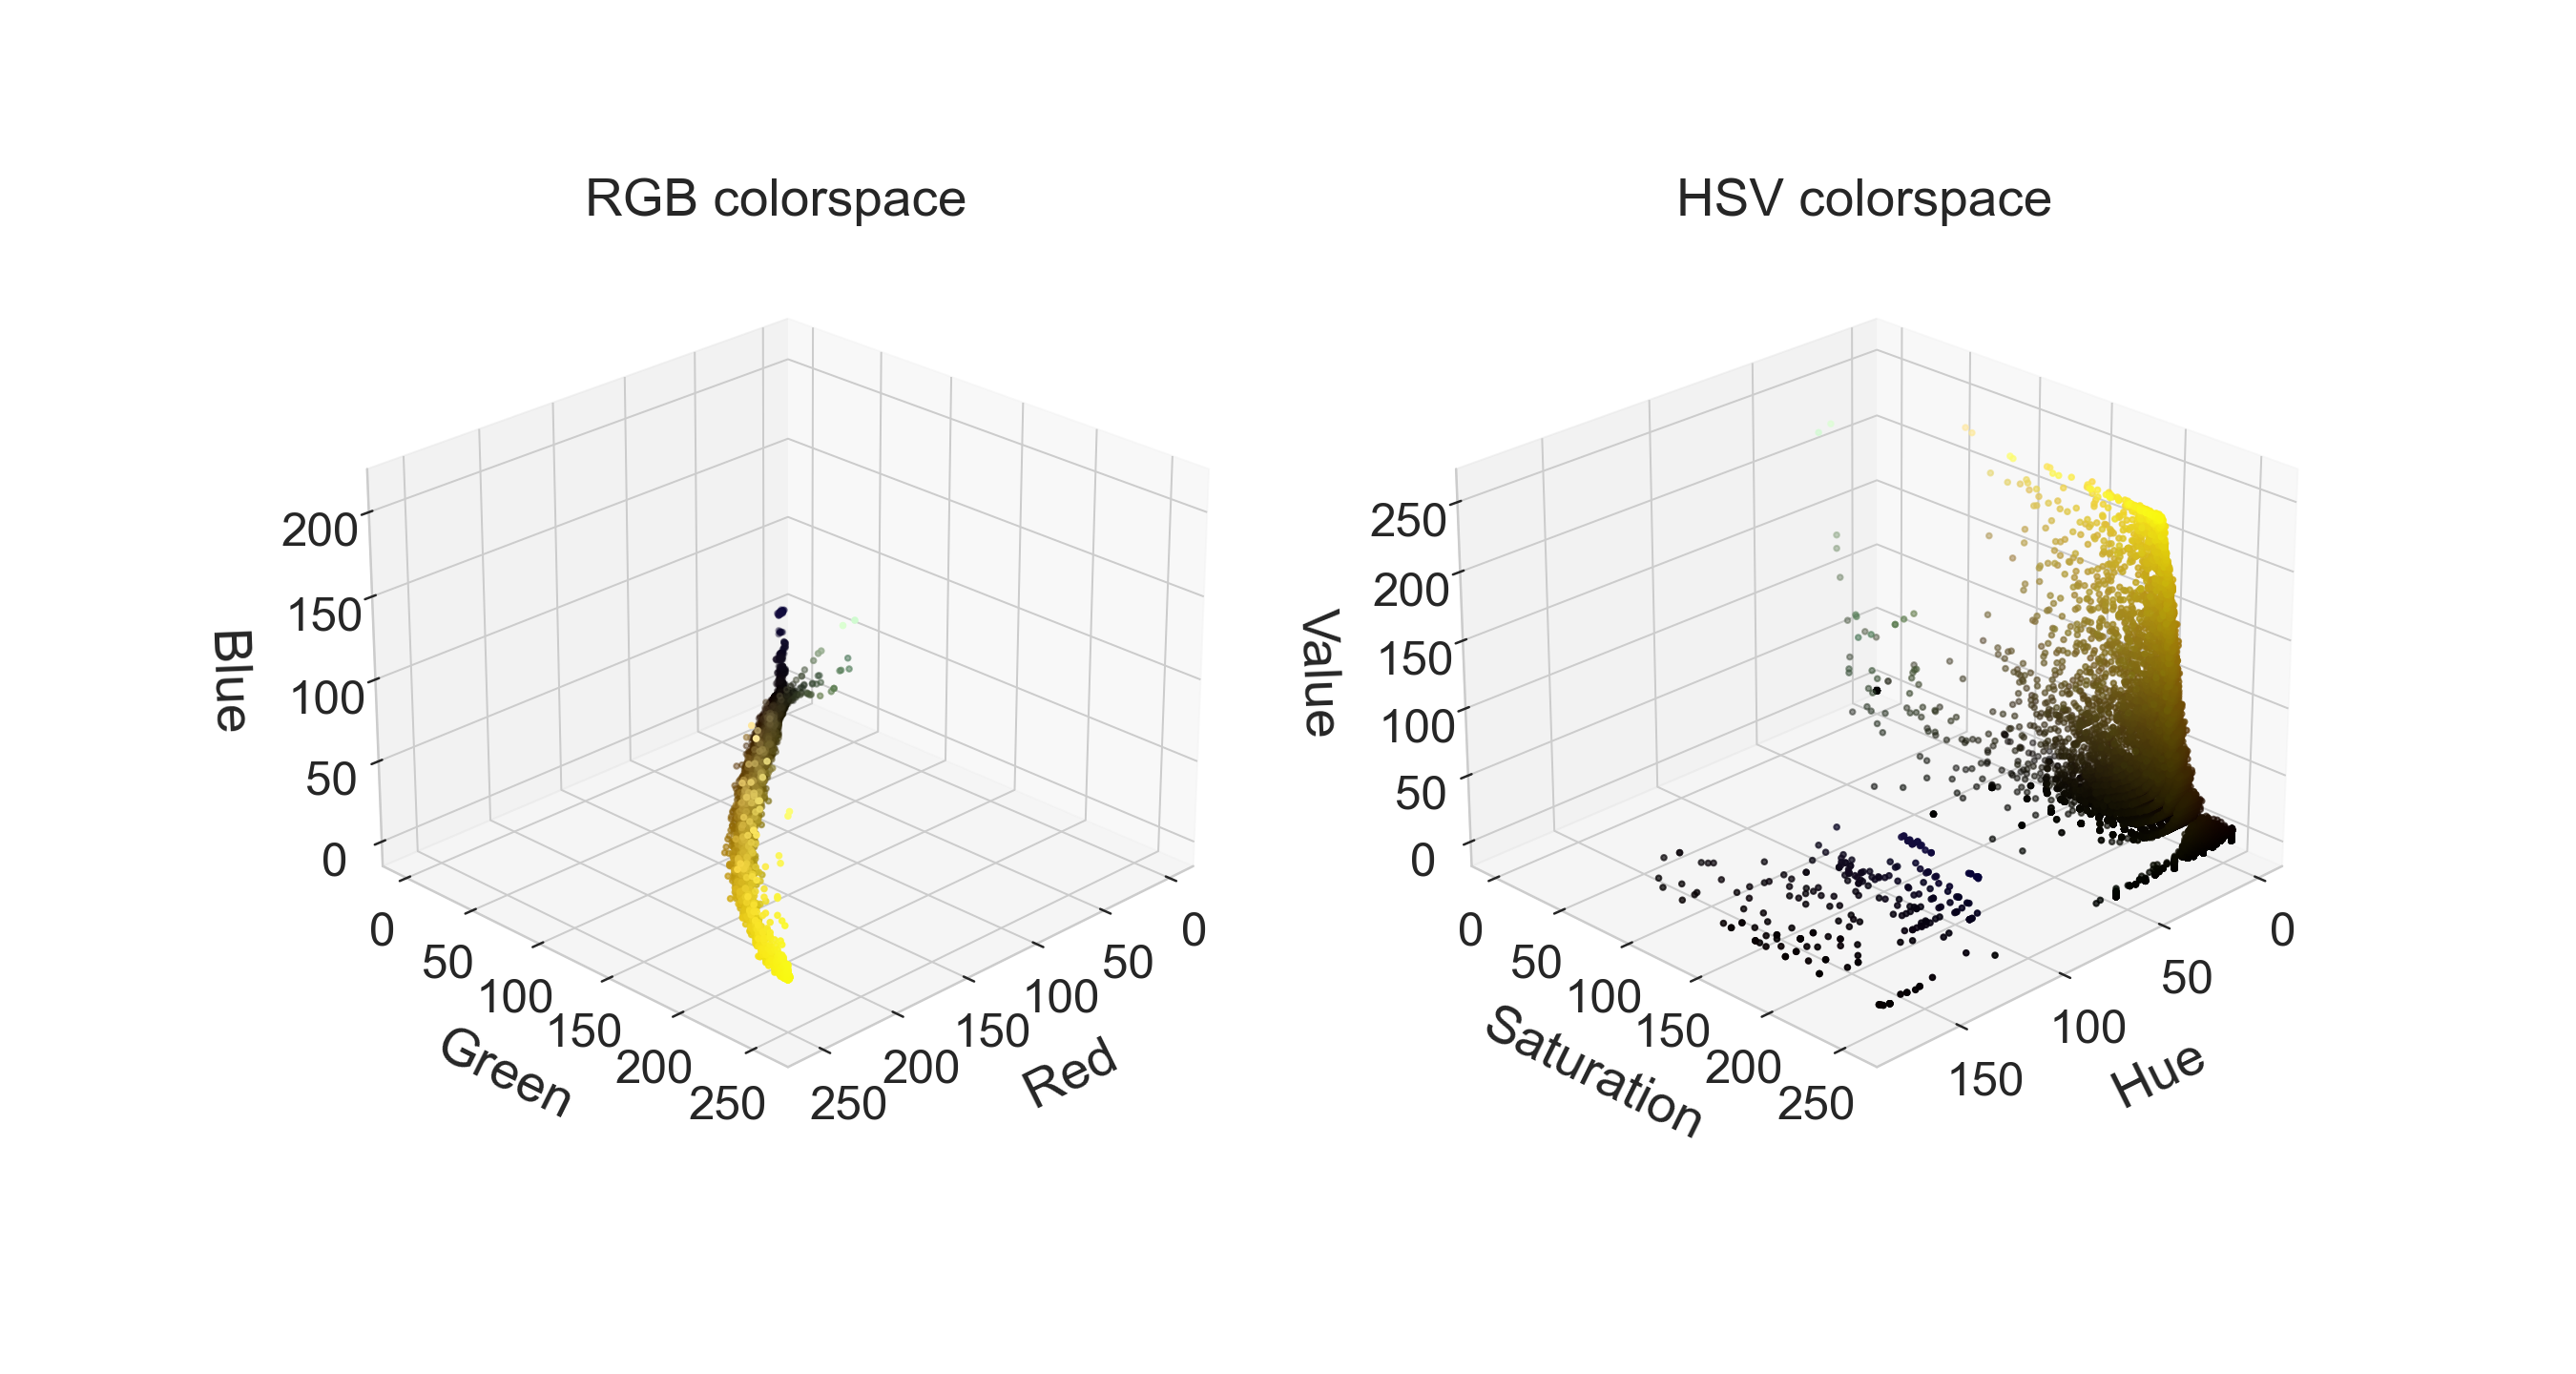
\includegraphics[width=1.1\textwidth]{figures/120_dataset/colorspace_Mar26bS2C1R2_DMl_200x_y.png}
    \caption{Colorspace representation. The same image is represented as RGB (left) and HSV (right). Pixels are treated as 3D points with coordinates given by their encoding in the corresponding colorspace}
    \label{fig:dataset:colorspace}
\end{figure}

\subsection{Class imbalance}


\subsection{Objects features}

